%!TEX root = ../deco_star.tex
\section{Introduction}
Pattern generation in computer graphics provides a large amount of precise and quickly-generated digital content. However, despite more than three decades of research, supporting artists with meaningful digital tools for creative content generation, \rev{Referencing a visual example:}{for example, those needed for ornamental pattern designs (\Cref{fig:historic_examples})}, is an ongoing challenge. Most solutions focus on singular features and control mechanisms, such as example-based controls or brushes, on an algorithmic level. Little attention, however, has been paid to overall creative workflows, which need to strike a balance, giving users needed power without burdening them with unwanted details. Often, techniques that are claimed to be artist-controllable turn out not to be so.

This may be a consequence of research often being executed without direct and continuous collaboration with artists and without the support of large-scale user studies. Algorithms and methods are often developed to further the state of the art, such as building on recent progress in deep learning research, with little understanding of artists' needs and how mechanisms can be validated.

Recent surveys have covered 3D generation in great detail, focusing on  world building~\cite{smelik_2014_aso, aliaga_2016_ipm}, terrain modeling~\cite{galin_2019_aro} and game-specific approaches~\cite{hendrikx_2013_pcg, togelius_2011_sbp}. In this report, we review recent advances in 2D pattern generation. 

The underlying regularity of 2D pattern designs is based on a repetitive and balanced distribution of elements, usually following hierarchical structures. These characteristics can be efficiently implemented by procedural approaches that arrange elements in space according to generative rules~\cite{stava_2010_ipm}, but developing these rules can be tedious, non-inspiring, repetitive, and challenging. The primary motivation for inverse procedural models is to free the artist from these tasks. Computational generation techniques can ease these problems and also perform in a more precise and less error-prone way than a human artist. \revremove{Condensing}{Hence, procedural representations are an ideal basis for creative pattern generation.}However, the creative demands of tasks like laying out space-specific designs and placing visual accents must also be considered. Procedural models must be augmented and different approaches must be unified to combine the control and quality of manual creation with the efficiency and accuracy of computation~\cite{gieseke_2017_ooo}. 

We review recent advances in 2D pattern generation and discuss procedural models, data-driven generation, and design-specific pattern generation. As theoretical grounding, we classify control mechanisms and their characteristics from the perspective of an artist, from global to local and from automatic to manual, with varying levels of abstraction. As a basis for a discussion of the capabilities of control mechanisms in the creative process and their potential for innovative creation, we review relevant literature on creativity and summarize aspects that can help to understand these capabilities in the context of computer graphics research.

We organize contemporary techniques by design areas and the visual features they enable. We further group related work by commonly-used control types. Then, we specifically analyze the artistic controls offered by each technique. 
We conclude the review with a discussion of the means for enabling creativity for the different control mechanism types. With this survey, we hope not only to meaningfully categorize and summarize the state of the art but also to contribute to a shared vocabulary and to establish a foundation for incorporating artists and their creative tasks into algorithmic content creation pipelines.

\begin{figure}
    % \centering
        %TODO: Replace with png for submission
        \revimage{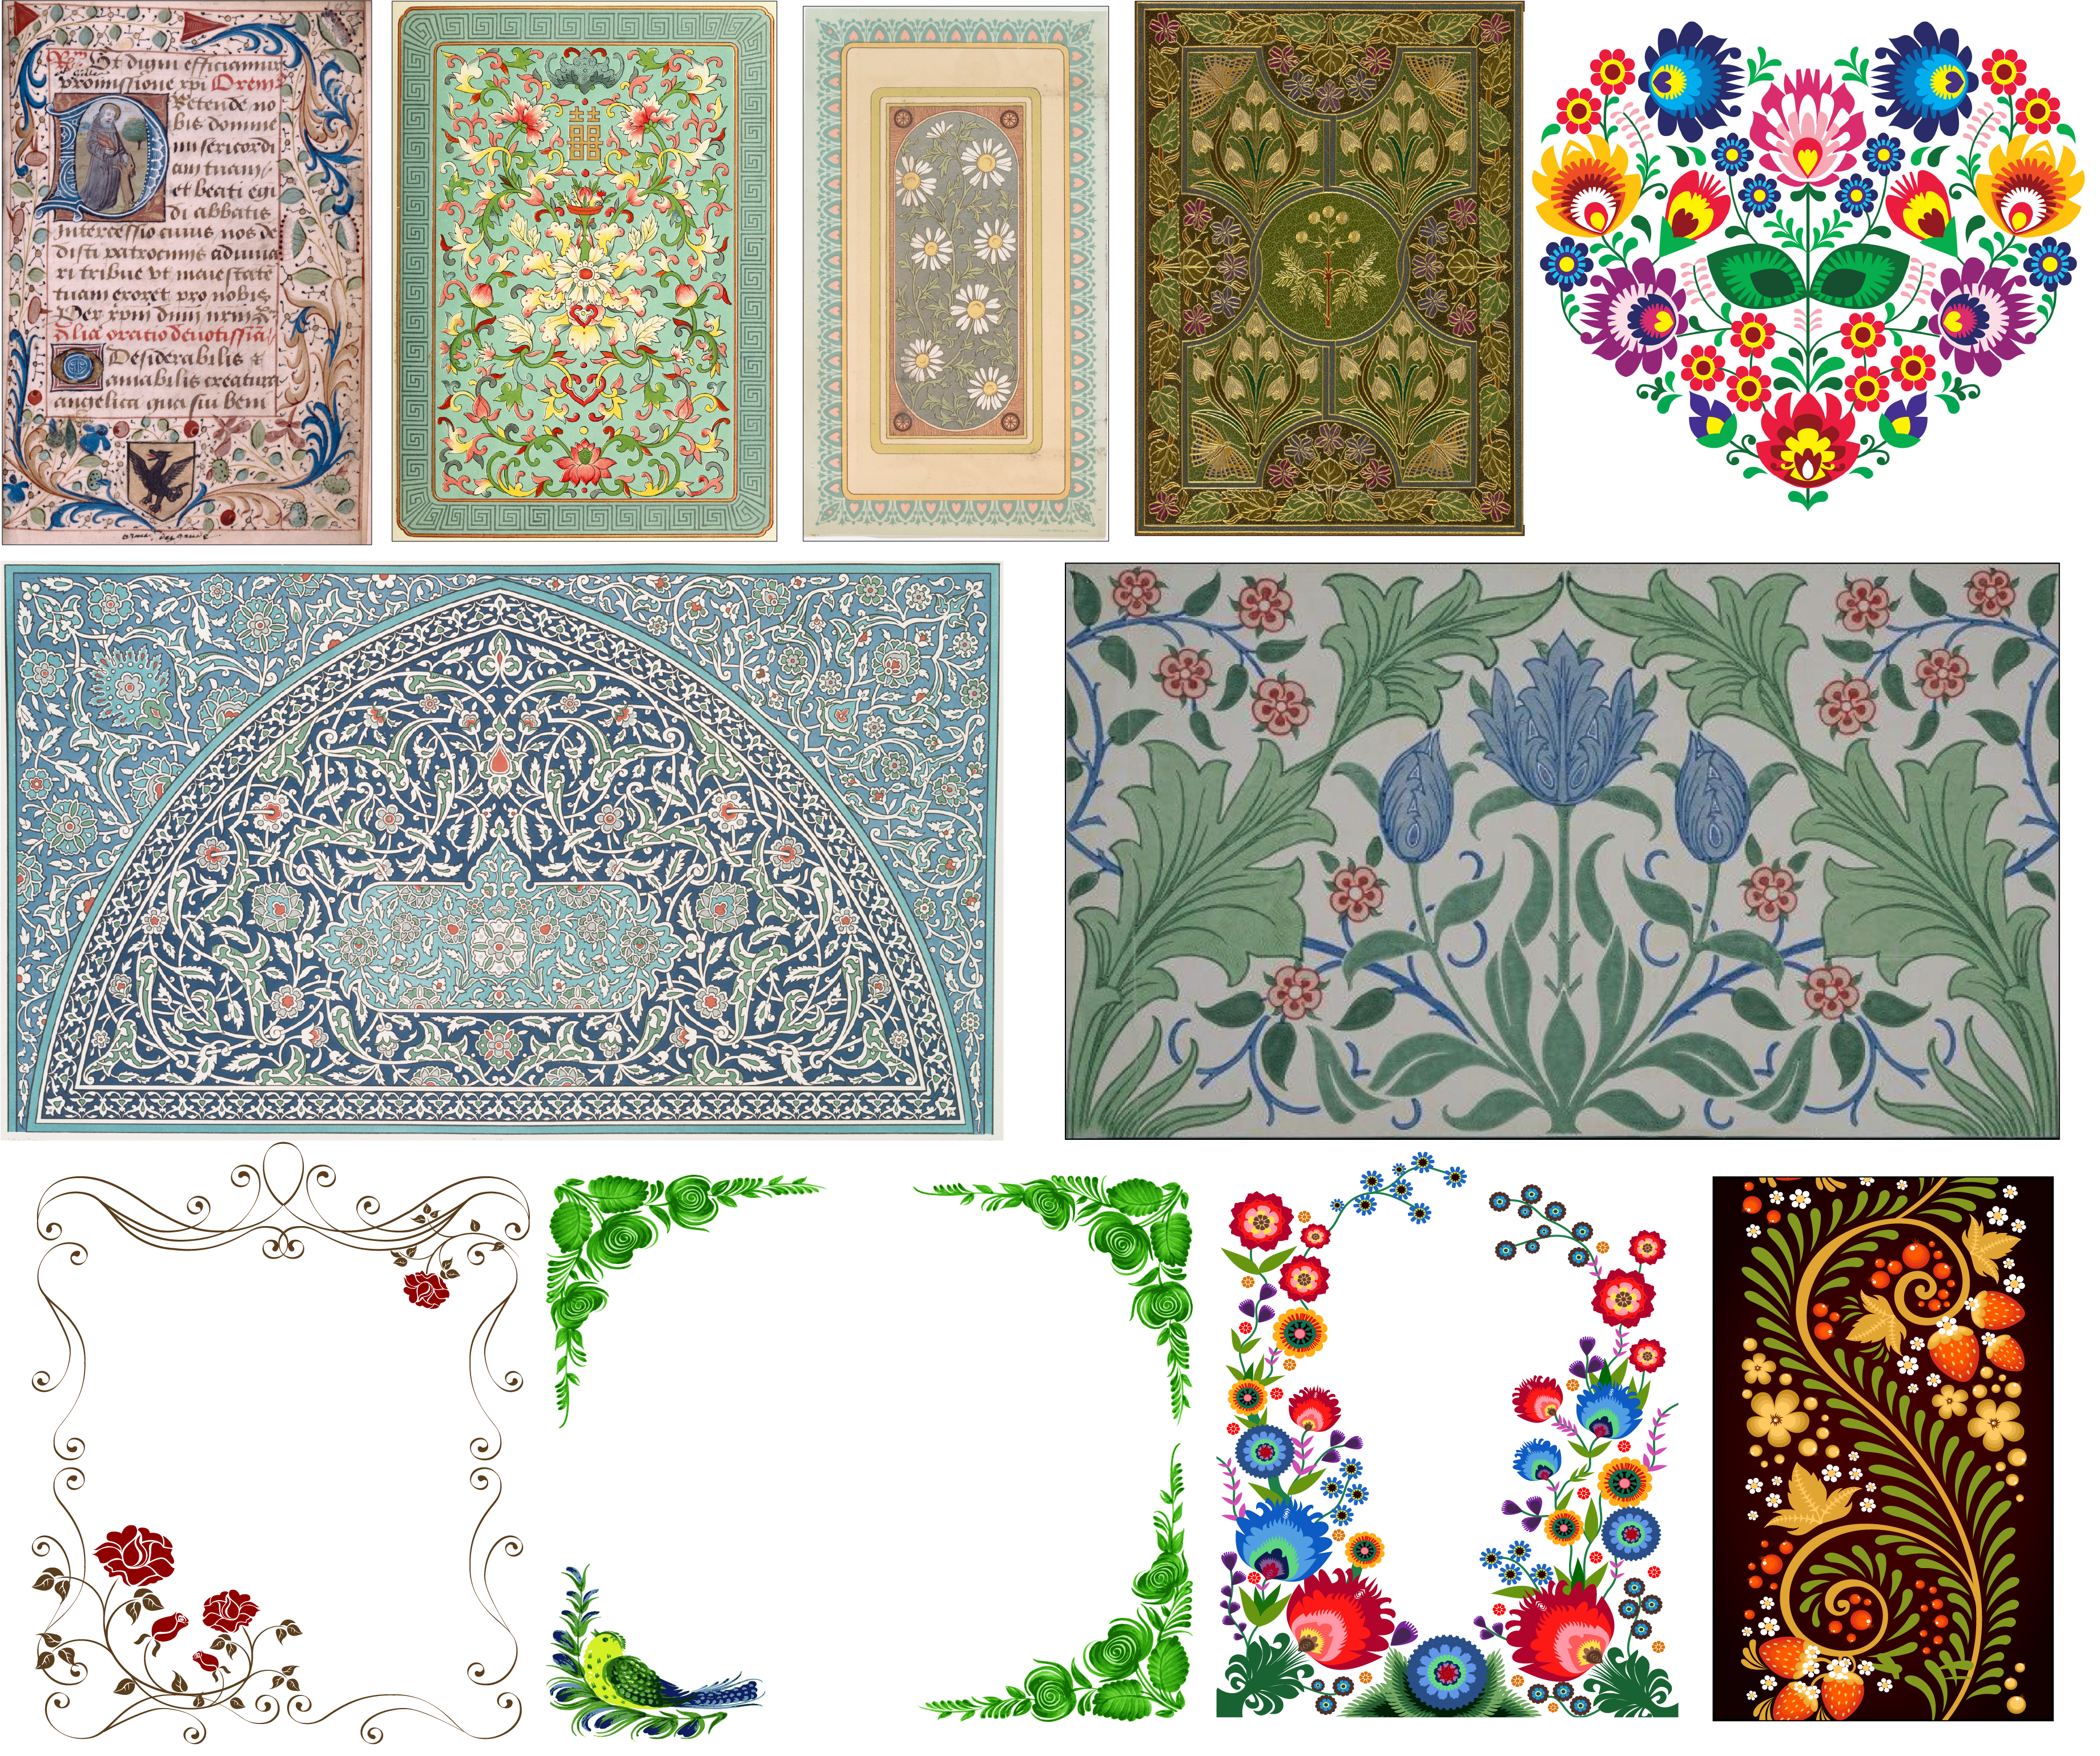
\includegraphics[width=1.0\columnwidth]{figures/historic_examples/examples.png}}
        \caption[Historic pattern examples]{\label{fig:historic_examples} Historic examples for creative pattern designs and ornamentation. Places of origin from left to right, top to middle row:  France, China, USA, UK, Poland, Egypt, UK. Bottom row: recent commercial examples. This figure is adapted from~\cite{gieseke_2017_ooo}, image sources: [1-11].}
\end{figure}
